\chapter{РЕАЛИЗАЦИЯ СИСТЕМЫ УПРАВЛЕНИЯ РОБОТОМ ГЕКСАПОДОМ}
   
В этой главе описывается этап реализации системы управления роботом-гексаподом на основе спроектированной во второй главе архитектуры. Рассматриваются необходимые компоненты, их связь друг с другом, а также  принцип работы и примеры.

\section {Sketch}

Для проектирования и визуализации UI (User Interface) веб версии пульта управления роботом был выбран Sketch – векторный графический редактор для macOS, разработанный голландской компанией Bohemian Coding, предназначенный исключительно для создания интерактивных прототипов веб-приложений и дизайнов приложений. Основные преимущества и недостатки данного редактора отражены в таблице \ref{tab:sketch} В отличие от Photoshop, графическое программное обеспечение Sketch изначально создавалось для разработки интерактивных интерфейсов. Он создает живые композиции, чтобы была возможность просматривать, что происходит, когда пользователь щелкает, смахивает или касается нарисованного дизайна на своем настольном компьютере, ноутбуке, планшете или телефоне.

Проектирование дизайна веб-пульта для робота-гексапода изображено на рисунке \ref{img:sketch}.


\begin{table}[h!]
	\caption{Преимущества и недостатки Sketch}
	\label{tab:sketch}
	\begin{tabularx}{\textwidth}{|X|X|}
		\tabheader{Преимущества}{Недостатки}
		Интуитивный интерфейс & Только MacOS\\\hline
		Быстрое обучение & Только одно устройство на одну лицензию\\\hline
		Полезные функции для совместной работы & Нет автоматической разметки\\\hline
		Работает с активами Illustrator & \\\hline
	\end{tabularx}
\end{table}

\begin{figure}[h!]
	\centering
	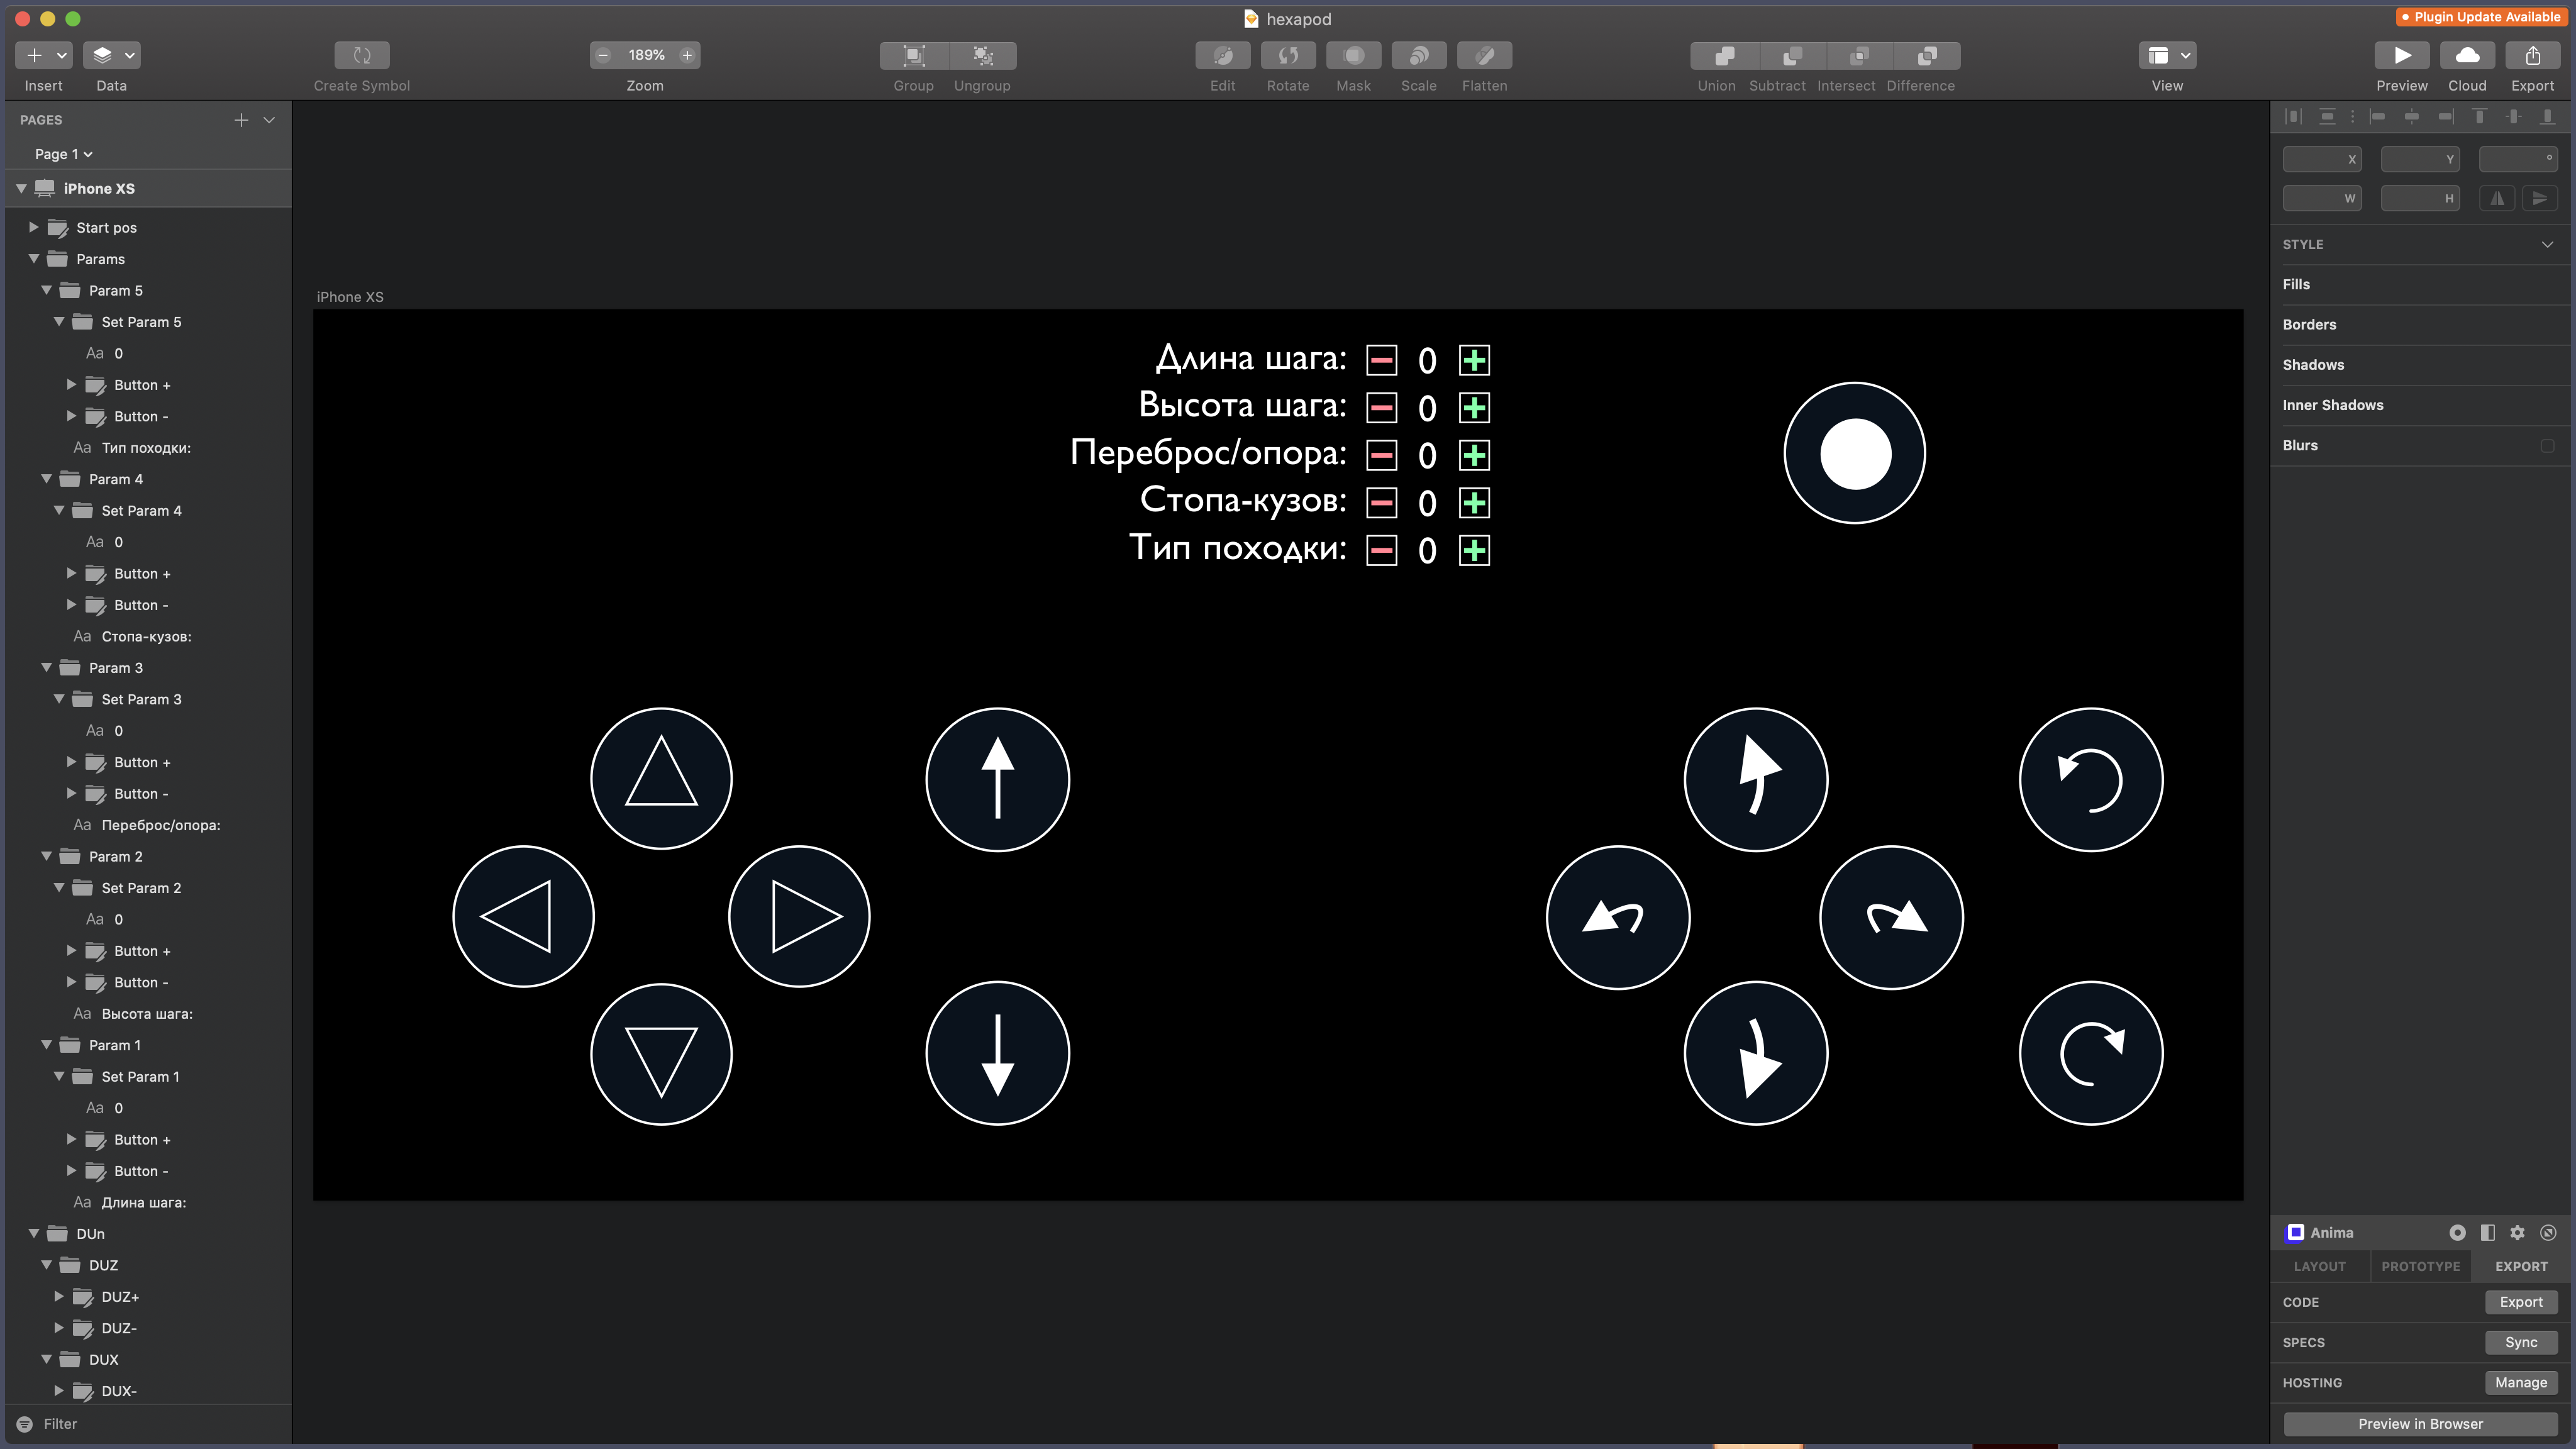
\includegraphics[width = \linewidth]{img/sketch}
	\caption{Проектирование Web UI пульта управления в Sketch}
	\label{img:sketch}
\end{figure}

\section{Front-end и VueJS}

Для реализации веб интерфейса управления был выбран Vue – современный javascript фреймворк. На первый взгляд, можно сказать, что библиотека Vue - это просто смесь Angular и React. Фактически, Evan You, создатель Vue, заимствовал концепции из Angular и React. Например, концепция использования Vue предполагает сохранение логики и макетов компонентов вместе с таблицами стилей в одном файле. Это похоже на то, как React работает без таблиц стилей. Чтобы позволить компонентам Vue общаться друг с другом, Vue использует реквизиты и объекты состояния. Этот подход также существовал в React до того, как Vue приняла его.

Как и в Angular, во Vue предполагается смешивание макетов HTML с JavaScript. При верстке необходимо использовать директивы Vue, такие как v-bind или v-if, чтобы интерполировать значения из логики компонента в шаблоны.

Одна из причин, по которой Vue стоит рассматривать вместо React, заключается в том, что библиотека Redux часто используется в крупномасштабных приложениях React. Как объясняется в разделе React, когда приложение React + Redux становится больше, требуется тратить много времени на внесение небольших изменений в несколько файлов вместо того, чтобы фактически работать над функциями. Библиотека Vuex - Flux-подобный инструмент управления состоянием, разработанный для Vue кажется менее громоздким, чем Redux.

Что касается выбора между Vue и Angular, причины выбора Vue вместо Angular могут быть сведены к следующему: Angular - это слишком сложная, полноценная структура с ограничительным характером; Vue намного проще и менее строг, чем Angular.

Также стоит отметить, что для использования Vue по сравнению с Angular и React, не требуется изучать ничего кроме JavaScript. Vue не требует другой расширенный набор JavaScript, такой как TypeScript (для Angular) или JSX (для React). В результате обучение работе с Vue быстрее, чем с Angular и React.

Одним из недостатков Vue является то, что он все еще гораздо менее популярен, чем React или Angular. Хорошим показателем использования инфраструктуры JS является количество вопросов, возникающих на Stack Oveflow. Вопросы показывают, с какими фреймворками чаще всего сталкиваются разработчки, хотя это также говорит об их уровне сложности.

В этом случае впервые в истории вопросы в 2019 году по React слегка опередили вопросы по Angular. Между тем, вопросы Vue имеют тенденцию к росту, но все еще остаются низкими. Статистика по вопросам использования Angular.js (старой версии) упала, как и ожидалось. Статистика вопросов по Javascript front-end фрейворкам изображена на рисунке \ref{img:vuejsstat}. Таким образом, у Vue гораздо меньше готовых решений, поэтому при решении нетривиальных задач приходится тратить немного больше времени на разработку. 

\begin{figure}[h!]
	\centering
	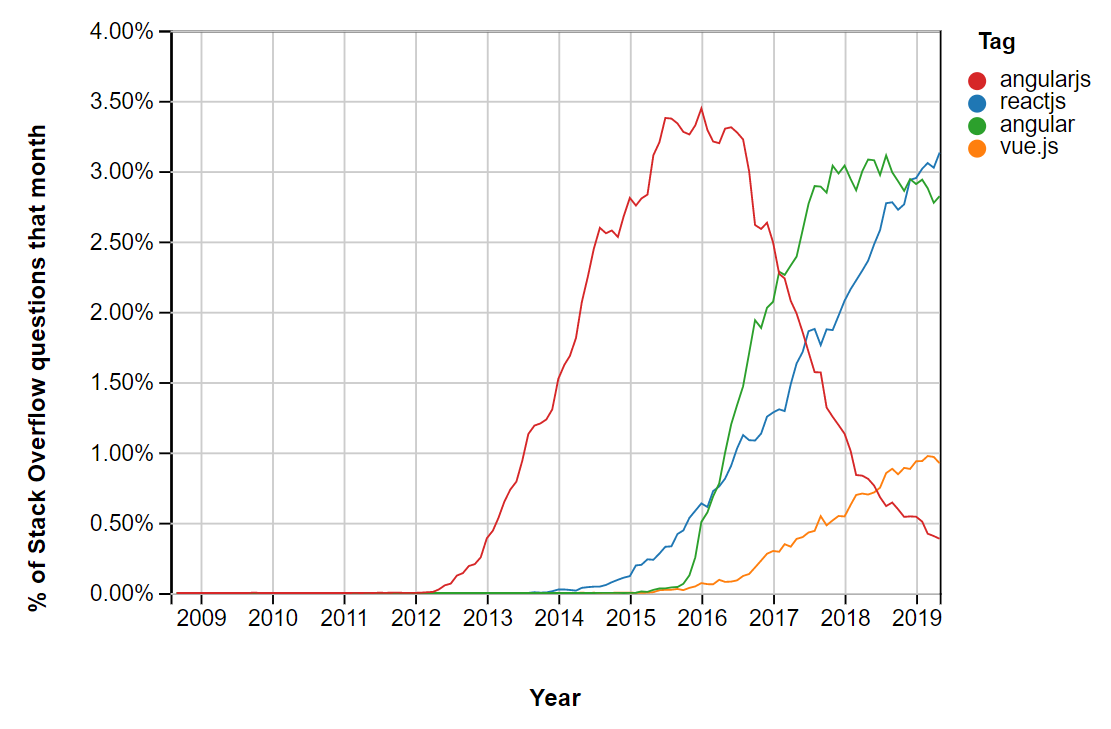
\includegraphics[width = \linewidth]{img/vuejsstat}
	\caption{Статистика вопросов по JS front-end фреймворкам на Stack Overflow}
	\label{img:vuejsstat}
\end{figure}

Экосистема VueJS состоит из:

\begin{itemize}
	\item Vue как библиотека представления;
	\item Vue-загрузчик для компонентов;
	\item Vuex, выделенная библиотека для управления состоянием приложения с помощью Vue, Vuex близок по концепции к Flux;
	\item Vue.js devtools для Chrome и Firefox.
	\item Nuxt.js, проект, предназначенный для создания серверных приложений с помощью Vue. Nuxt.js является  конкурентом для Angular Universal;
	\item Weex, библиотека JS, которая поддерживает синтаксис Vue и используется для мобильной разработки.
\end{itemize}

\section{Browser-Sync}

BrowserSync - это инструмент автоматизации, который ускоряет веб-разработку, настройку и тестирование за счет синхронизации изменений файлов и взаимодействия на многих устройствах.

Особенности BrowserSync:

\begin{itemize}
\item Перезагрузка в реальном времени – это, вероятно, самая важная функция BrowserSync. При изменении кода страница автоматически перезагружается. Прямая перезагрузка работает во многих браузерах и устройствах;
\item Синхронизация взаимодействия –это означает, что все действия отражаются во всех браузерах. Эта небольшая функция полезна для тестирования, особенно при тестировании на многих устройствах. Также можно настроить, какие действия отражаются в разных браузерах;
\item Имитация более медленных соединений – используется для тестирования при интернет-соединении, благодаря тому, что BrowserSync имеет функцию, которую можно использовать для регулирования скорости соединения сайта;
\item История URL – BrowserSync регистрирует всю историю просмотров, чтобы можно было отправить тестовый URL на все устройства;
\item BrowserSync совместим со многими исполнителями задач, такими как GULP и Grunt. И они работают во многих операционных системах.
\end{itemize}

Принцип работы заключается в том, что BrowserSync создает небольшой сервер, но если уже имеется настройка сервера, BrowserSync может подключиться к этому серверу и действовать как прокси. Затем он вставляет файл javascript на каждую страницу. Этот файл использует WebSockets для связи между сервером и клиентом для отслеживания изменений в коде или действиях браузера. Как только BrowserSync обнаруживает действие, он выполняет перезагрузку страницы.


\section{ROS}

ROS (Robot Operating System) предоставляет стандарт для разработки программного обеспечения для робототехники, который можно использовать с любым роботом. Этот стандарт позволяет фактически сосредоточиться на ключевых функциях приложения, используя существующую основу, таким образом реализуя middleware слой.

ROS в основном разработан с использованием 2 языков: C++ и Python. Это часто наиболее предпочтительные и используемые языки при разработке приложений для робототехники. Библиотека roscpp используется для написания кода на C++, а библиотека rospy для написания кода на Python. Есть также несколько библиотек для создания моста с другими языками, такими как rosjava для Java и roslibjs или rosnodejs для JavaScript.

С помощью ROS можно легко разделить кодовую базу на пакеты, содержащие небольшие программы, называемые узлами. Для передачи данных между этими узлами ROS содержит 3 основных средства коммуникации:

\begin{itemize}
	\item Топики используются в основном для отправки потоков данных между узлами. К примеру, отслеживаются некоторые параметры на роботе. Узел, контролирующий эти параметры, отправит поток данных с этими параметрами. Теперь любой другой узел может подписаться на этот топик и получить данные (рис. \ref{img:topic});
	\item Сервисы позволят создать простую синхронную клиент-серверную связь между узлами. Используется для изменения настроек робота или для запроса определенного действия: включить режим походки, запросить определенные данные и так далее;
	\item Действия основаны на топиках. Они предназначены для того, чтобы предоставить асинхронную архитектуру клиент / сервер, где клиент может отправить запрос, который занимает много времени (например, запросить перемещение робота в другое место). Клиент может асинхронно отслеживать состояние сервера и отменять запрос в любое время.
\end{itemize}

\begin{figure}[h!]
	\centering
	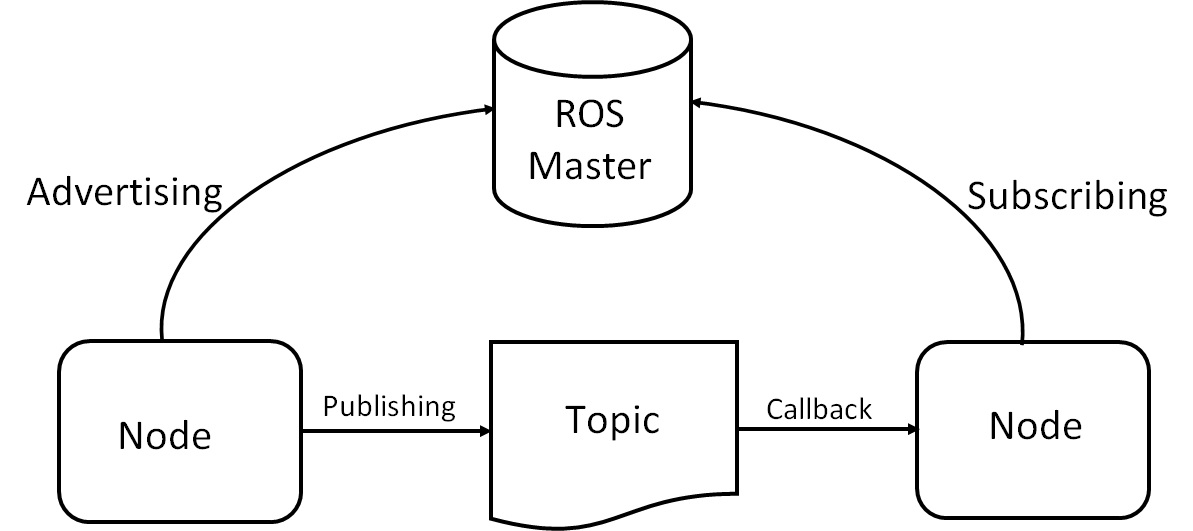
\includegraphics[width = 0.8\linewidth]{img/topic}
	\caption{Топик как способ коммуникации между двумя и более узлами}
	\label{img:topic}
\end{figure}

При создании топика необходимо указать тип сообщений (messageType) который будет передаваться с его помощью. В ROS существуют встроенные типы сообщений, однако этого не всегда бывает достаточно, поэтому имеется возможность создания кастомных сообщений по необходимости. В данной работе дополнительно был создан FrundControl, для передачи параметров управления от пульта, листинг приведен ниже.

\begin{lstlisting}[frame=single]
# Hexapod walking parameters
# accel           Control movement and rotation
# gait_settings   Extra gait settings

geometry_msgs/Accel accel
hexapod_msgs/GaitParams gait_settings
\end{lstlisting}

В данном случае accel представляет собой стандартный тип сообщений, содержащий в себе ускорение в свободном пространстве, разбитое на его линейную и угловую части:

\begin{lstlisting}[frame=single]
# This expresses acceleration in free space broken into 
# its linear and angular parts.
Vector3  linear
Vector3  angular
\end{lstlisting}

где linear и angular представляет собой:

\begin{lstlisting}[frame=single]
float64 x
float64 y
float64 z
\end{lstlisting}

Gait\_settings также является кастомным сообщением, входящим в состав FrundControl и содержит в себе дополнительные настраиваемые параметры походки:

\begin{lstlisting}[frame=single]
# Extra gait settings for FRUND gait generator

float32 step_length
float32 step_height
float32 support_movement
float32 foot_body_ratio
uint8   gait_type
\end{lstlisting}


Стоит отметить, что ROS не зависит от языка. Написанные подпрограммы (узлы) могут быть написаны на любом языке. Таким образом, приложение может иметь узел, написанный на Python, взаимодействующий с узлом, написанным на C++ (рис. \ref{img:roslang}). Это является возможным, благодаря тому, что уровень коммуникации ниже "языкового уровня"{}. Поскольку он работает как middleware ПО, используются стандартные сокеты TCP / IP для связи между узлами.

\begin{figure}[h!]
	\centering
	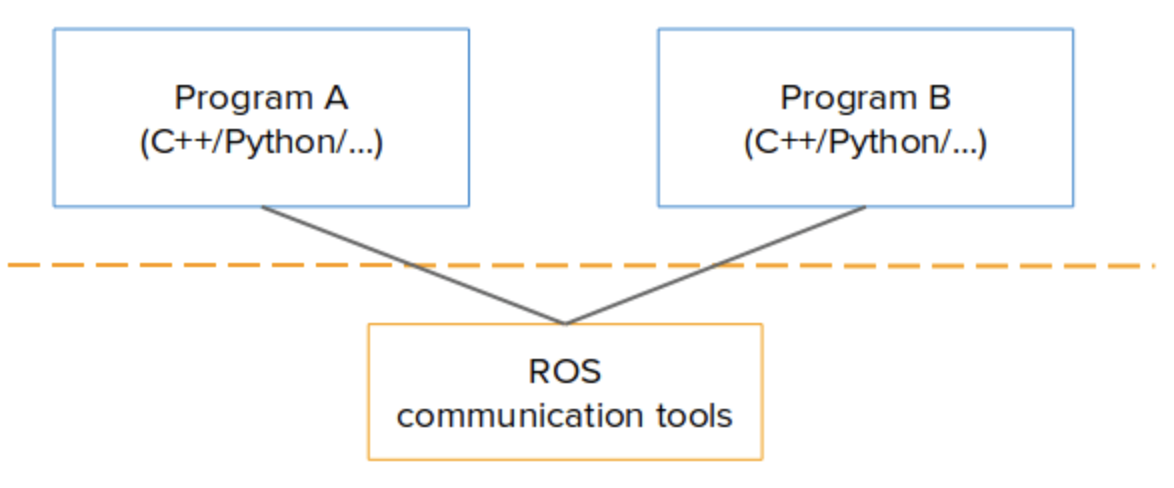
\includegraphics[width = 0.8\linewidth]{img/roslang}
	\caption{Работа слоя коммуникации ROS}
	\label{img:roslang}
\end{figure}

ROS не заканчивается набором основных функций и средств коммуникации. Одним из главных преимуществ является возможность использования огромного количества существующих библиотек. Для большинства общих блоков разработки в робототехнике можно найти ROS-пакет с открытым исходным кодом. Пример использования и связи различных компонентов в ROS представлена на рисунке \ref{img:rospackets}.

\begin{figure}[h!]
	\centering
	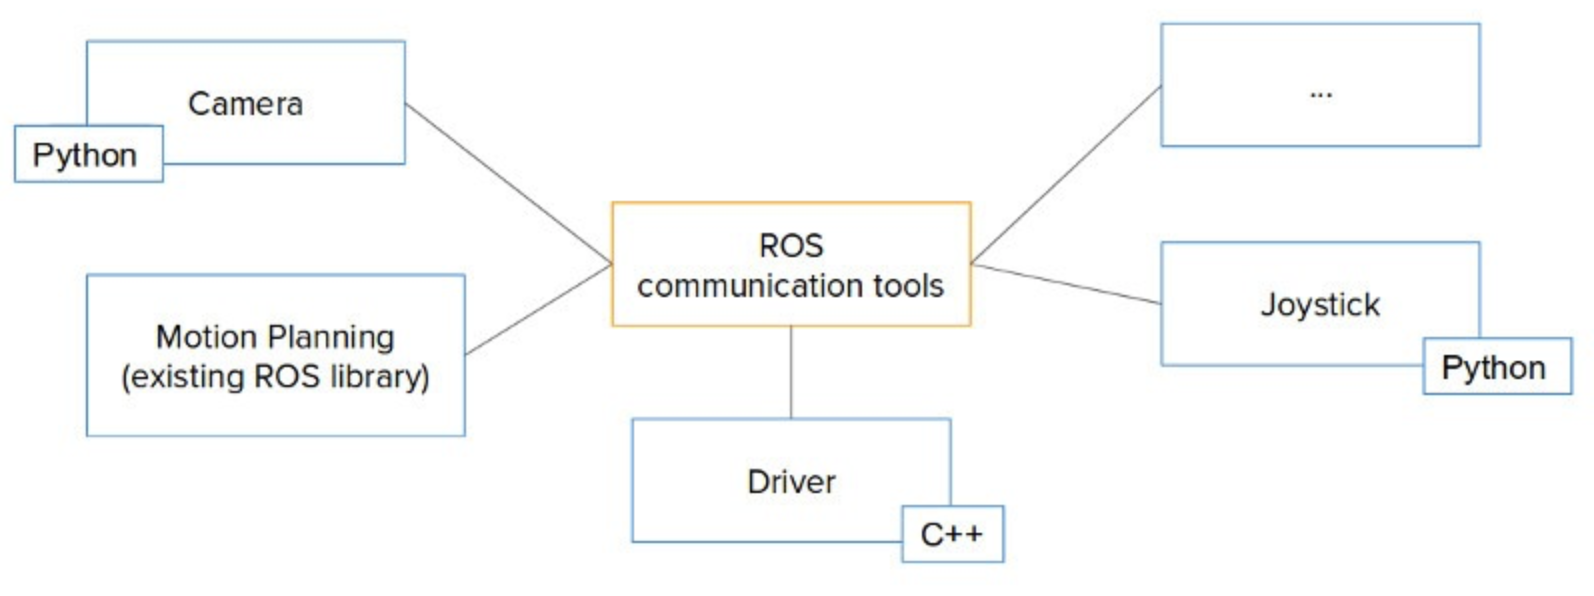
\includegraphics[width = \linewidth]{img/rospackets}
	\caption{Связь между узлами в ROS}
	\label{img:rospackets}
\end{figure}

Пример используемых библиотек / пакетов:

\begin{enumerate}
	\item Многие двигатели и камеры имеют существующий драйвер ROS;
	\item Для основного цикла управления робота используется ros\_control;
	\item Чтобы представить трехмерную модель вашего робота, требуется описать ее, используя XML с форматом URDF;
	\item Для планирования пути и движения используется Moveit. Moveit будет использовать ранее созданный  файл URDF;
	\item Для перемещения мобильного робота вы можете найти полный стек навигации;
	\item Для 3D визуализации используется Rviz;
	\item Если требуется более мощный инструмент моделирования с физическими ограничениями, к примеру, с гравитацией и ветром то стоит использовать GAZEBO;
	\item Для возможности обмениваться данными между ROS и окружением без ROS используется пакет rosbridge. 
\end{enumerate}

Для визуализации графа ROS приложения используется rqt\_graph - это графический плагин из набора инструментов Rqt.

В окне rqt\_graph можно сразу увидеть все работающие узлы, а также связь между ними. Узлы и топики будут отображаться в их пространстве имен. Стоит отметить, что службы ROS в графике rqt не отображаются, только топики (рис. \ref{img:rqt}). Это связано с тем, что они были реализованы как сервисы.

\begin{figure}[]
	\centering
	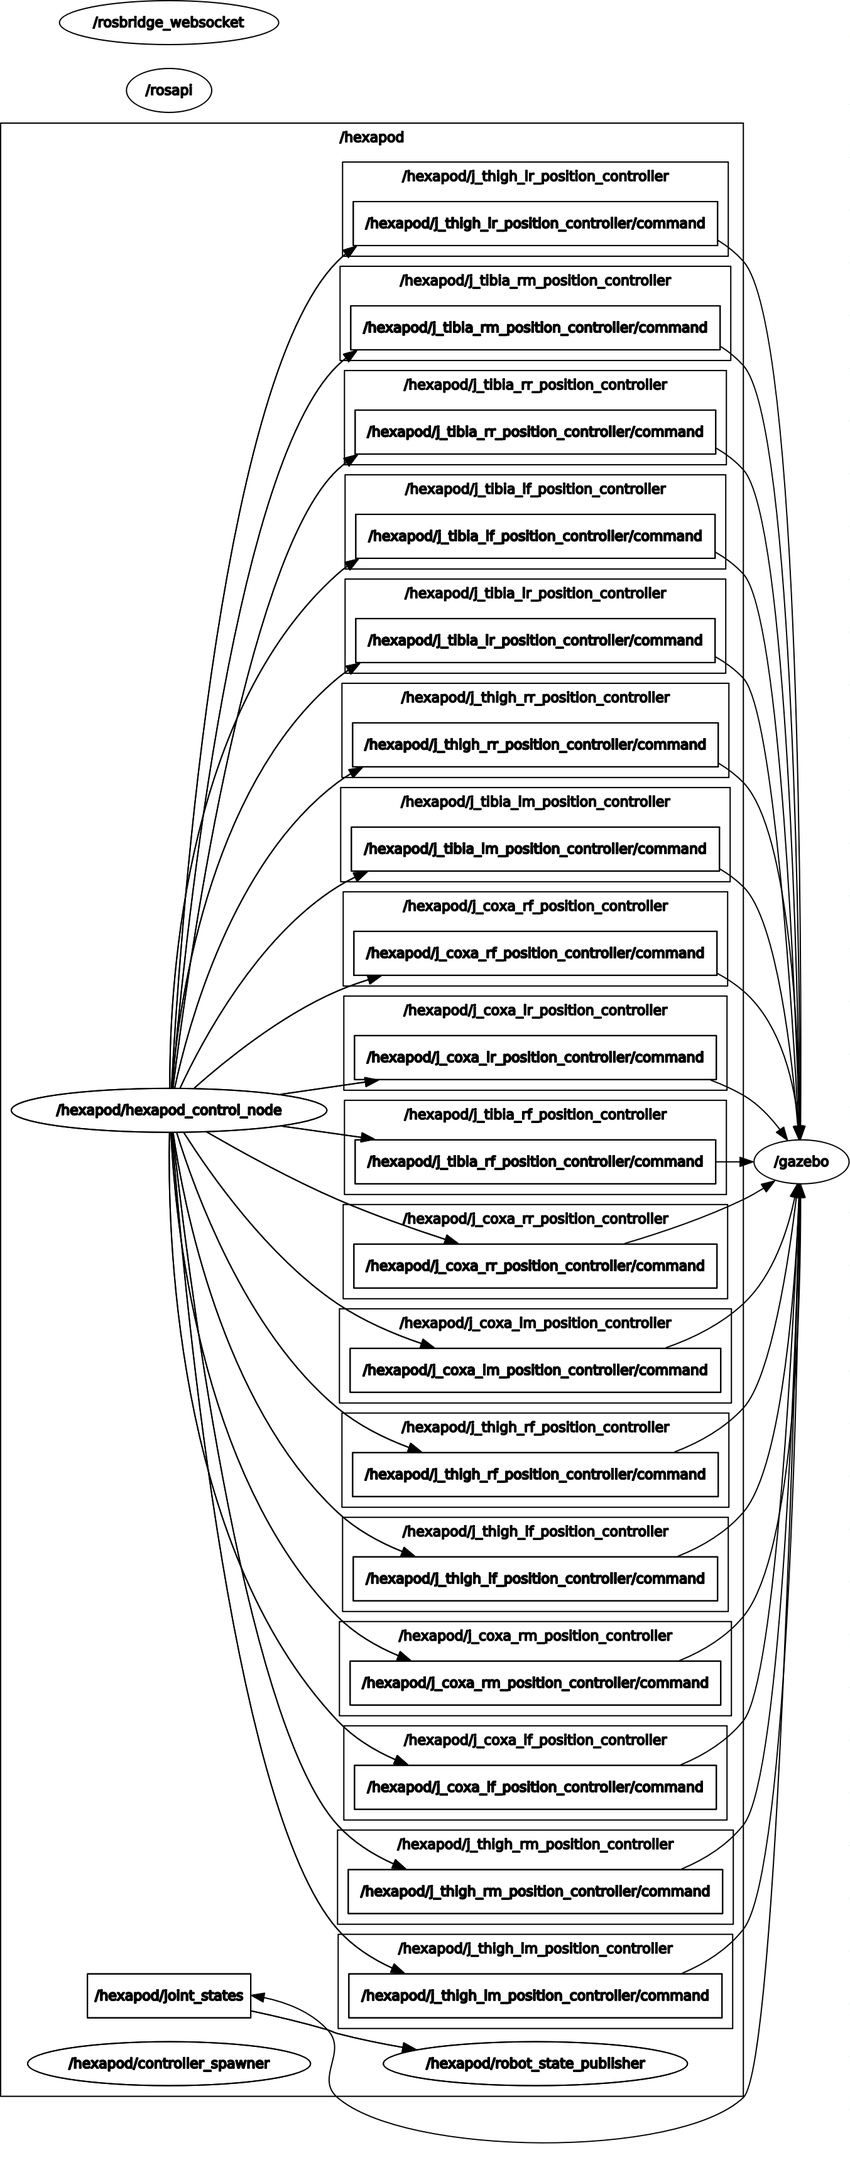
\includegraphics[height = 0.9\textheight]{img/rqt}
	\caption{Вывод rqt\_graph для системы управления роботом-гексаподом}
	\label{img:rqt}
\end{figure}

Рассмотрим компонент FRUND bridge, также реализуемый в рамках реализации данной системы управления.
Диаграмма классов данного компонента приведена на рисунке \ref{img:frundb_class}.

\begin{figure}[h!]
	\centering
	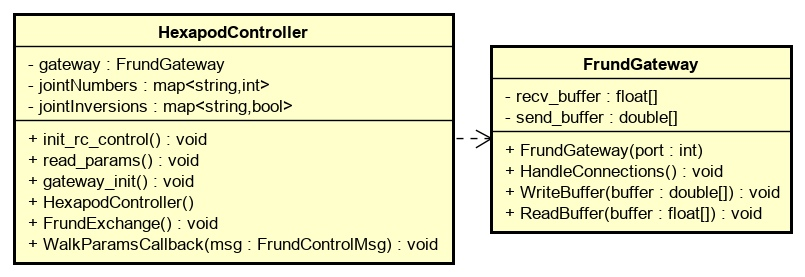
\includegraphics[width = \linewidth]{img/frundb_class}
	\caption{Диаграмма классов компонента FRUND bridge}
	\label{img:frundb_class}
\end{figure}

Диаграмма класов включает в себя два класса, первый из которых (HexapodController) выполняет общие операции взаимодействия с гексаподом и прием данных с пульта. Второй класс (FrundGateway) является шлюзом между ROS топиками и системой ФРУНД. Экземпляр FrundGateway используется в HexapodController для организации передачи управляющих траекторий приводов с ФРУНД в топики, которые сообщают положения joint в ROS control и для передачи управляющих параметров движения (команд) с пульта к системе ФРУНД.

Метод init\_rc\_control выполняет настройку подписчика ros\_subscriber для приема команд из топика, когда приходит очередная порция команд, вызывается функция обратного вызова WalkParamsCallback в которой принятые параметры записываются в буффер для передачи системе ФРУНД. Метод read\_params читает данные (словарь параметров соотвествия между joint ROS и каналами во ФРУНД, номер порта, для соединения с ФРУНД по поотоколу UDP). Метод FrundExchange представляет собой итерацию обмена данными между ROS и сокетом, который, соединен с системой ФРУНД.

Для обмена данными по сокетам используются два буфера (класс FrundGateway). recv\_buffer принимает массив позиций приводов модели роботов с ФРУНД и затем они читаются в HexapodController с помощью метода ReadBuffer и считанные данные записываются в топики ROS. send\_buffer используется для отправки (записи) параметров движения (команд) и данные в него заносятся из HexapodController за помощью метода WriteBuffer.

В конечном итоге взаимодействие между ФРУНД, пультом и моделью робота в ROS организуется путем итераций чтения данных с пульта, записи в буфер отправки, чтения данных с буфера приема, записи их в топики, и обменом буферами между запущенным шлюзом и системой ФРУНД по протоколу UDP по интерфейсу сокетов

\section{Rosbridge}

Rosbridge, представляет собой middleware слой абстракции программного обеспечения, предназначенный для разработки приложений, которые напрямую не связаны с роботом. Rosbridge предоставляет простой программный доступ на основе сокетов к интерфейсам и алгоритмам роботов, которые предоставляет ROS. В частности, это облегчает использование веб-технологий, таких как Javascript, с целью расширения использования и полезности роботизированных технологий.

Вычислительные парадигмы с течением времени развивались от автономных настольных систем до клиент-серверных архитектур и от повсеместных веб-приложений. Современные технологии обеспечивают прозрачное администрирование, избыточное хранилище и мгновенное развертывание программного обеспечения, работающего на сильно разнородных платформах, от смартфонов до многоядерных настольных компьютеров.

Поскольку rosbridge был создан для связи ROS и non-ROS приложений существует библиотека rosbridge в Javascript, известная как rosjs. Ее единственная расширенная зависимость - это технология веб-сокетов HTML5. В настоящее время такие браузеры, как Safari, Opera и Chrome, полностью поддерживают их. Rosjs реализован в виде простой библиотеки Javascript, полностью независимой от предпочтительных сред разработки. Rosbridge построен с использованием сериализованных объектов JSON, которые сами по себе являются базовым синтаксисом объектов Javascript.

В настоящее время rosjs - это большая библиотека, поддерживающая множество сложных функций для визуализации и взаимодействия со сложными алгоритмами манипулирования и навигации на основе ROS. Однако его можно использовать и для управления роботом посредством предоставления пользователю web интерфейса управления (рис. \ref{img:rosbridge}).

\begin{figure}[h!]
	\centering
	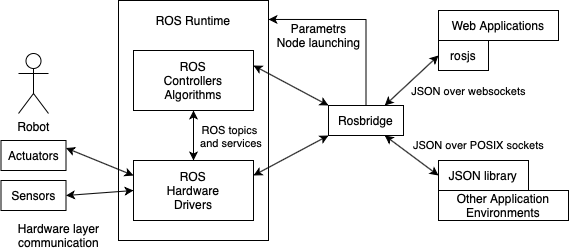
\includegraphics[width = \linewidth]{img/rosbridge}
	\caption{Rosbridge: ROS для non-ROS приложений}
	\label{img:rosbridge}
\end{figure}

\section{GAZEBO}

Симуляция робота является важным инструментом при разработке. Хорошо продуманный симулятор позволяет быстро тестировать алгоритмы, проектировать роботов, проводить регрессионное тестирование и обучать систему искусственного интелекта с использованием реалистичных сценариев. Для симуляции походки робота-гексапода был выбран GAZEBO, который имеет возможность точно и эффективно моделировать роботов в сложных внутренних и наружных условиях.

Первым шагом в моделировании в ROS является создание трехмерной модели. 3D-модель может быть создана с помощью любого из инструментов моделирования, таких как Inventor, Fusion 360, 3dsMax. Когда модель готова, она экспортируется в формат stl для интеграции в среду ROS. 

Важно помнить, что все части робота, имеющие различную степень свободы передвижения, должны создаваться отдельно. Например, при создании корпуса с звеньями ног их надо экспортировать отдельно, поскольку корпус статичен, а звенья ног динамичны и имеют определенную степень свободы для движения.

После создания трехмерных моделей отдельных компонентов они объединяются в ROS в окружения. Это возможно с помощью пакетной модели робота, которая содержит URDF-файлы синтаксического анализатора (Unified Robot Description Model). Также описания URDF связывают различные mesh (структурные сборки трехмерных моделей, состоящей из полигонов) через концепцию связей и соединений. Две части, соединенные joint (сустав / соединение), называются родительской и дочерней связью, а тип перемещения каждого элемента в модели определяется типом соединения между двумя связями. Тип joint может быть любым из следующих:

\begin{itemize}
	\item Fixed – как следует из названия, этот тип является фиксированным и не имеет никаких степеней свободы;
	\item Revolute – при данном типе есть возможность вращения вокруг оси, движение ограничено в указанных верхних и нижних пределах;
	\item Continuous – схоже с Revolute и также имеет возможность вращения вокруг оси, за исключением отсутствия границ;
	\item Prismatic – скольжение вдоль оси в указанных пределах;
	\item Planar – движение перпендикулярно указанной оси;
	\item Floating – все шесть степеней свободы свободны.
\end{itemize}

Файлы URDF содержат описание моделей и роботов для импорта в ROS. Такое описание включает в себя название объекта, его mesh-структуру, оболочку для расчета столкновения, дополнительную информацию о визуальных компонентах объекта, таких как цвет, текстура и другие. Рассмотрим более подробную композицию urdf-файла:

\begin{itemize}
	\item Тег <robot> содержит имя робота, которое будет отображаться во всех подсистемах ROS. Этот тег содержит описание всего окружения или его части (например, робота, объекта или датчика);
	\item Тег <link> также содержит имя и представляет визуальный компонент моделируемой среды или объект, который связан с другими объектами с помощью соединений (теги <joint>). Внутри тега <link> можно увидеть описание визуальной части модели (тег <visual>), которая содержит информацию о геометрии объекта <geometry>. Возможные значения – <cylinder>, <box>, <sphere> и <mesh>;
	\item Тег <origin> устанавливает начальную позицию объекта в пространстве.
	\item Тег <inertial> определяет массу объекта и смещенный центр масс внутри объекта. Он необходим для симуляции гравитации;
	\item Тег <collision> определяет параметры столкновения. Это возможно благодаря тому, что ROS создает невидимый слой поверх визуального объекта, который является оболочкой, имеющей возможность сталкиваться с другими объектами;
	\item Тег <joint> - это соединение между двумя частями объекта <link>. Тег <joint> содержит описание родительского объекта и дочернего объекта (их имен), тип соединения, то есть тип движения (revolute – вращение вокруг некоторой оси с верхним и нижним пределом, continuous – бесконечный поворот вокруг определенной оси без ограничений и другие виды движения), также есть информация о местонахождении joint и информация о контроллерах.
\end{itemize}

\begin{figure}[h!]
	\centering
	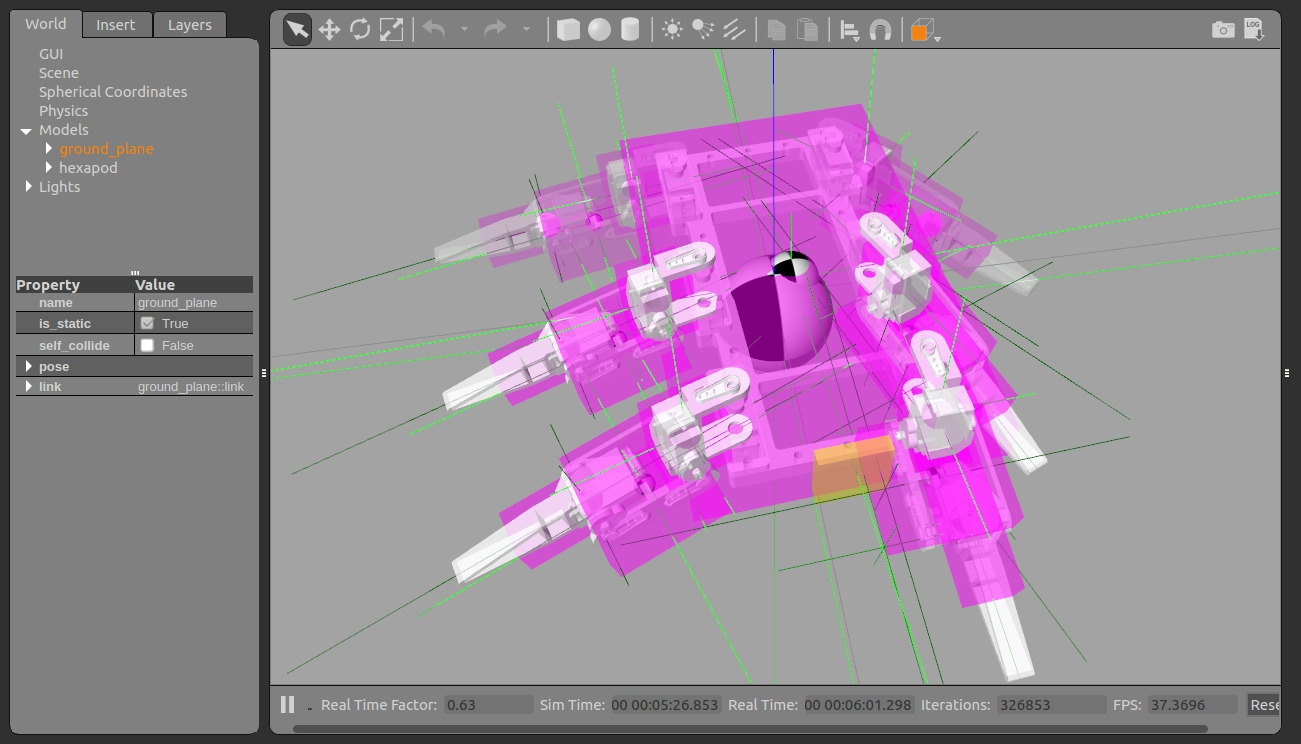
\includegraphics[width = \linewidth]{img/gazebocmi}
	\caption{Отображения моментов инерции и центра масс робота-гексапода в GAZEBO}
	\label{img:gazebocmi}
\end{figure}

Таким образом, файл URDF позволяет сделать полнофункциональную модель. Файл URDF обычно создается в текстовом редакторе. Конечно, в этом случае невозможно отслеживать в реальном времени изменения в трехмерном пространстве. Однако ROS имеет специальный пакет Rviz, который позволяет импортировать файлы URDF и показывает модель в трех измерениях. Кроме того, Rviz дает возможность манипулировать любыми объектами, входящими в среду. Например, перемещая ползунок, можно двигать ногами робота-гексапода. Rviz может анализировать столкновения и представлять их в виде трехмерной модели, отображать информацию о соединениях, массе и центре масс. Также некоторую информацию можно отображать и в GAZEBO (рис. \ref{img:gazebocmi}). Для запуска пакета Rviz необходимо создать файл запуска, в котором описаны все узлы и их параметры.

\section{Выводы по главе}

Таким образом, была разработана система управления инсектоморфным роботом-гексаподом, на основе архитектуры, спроектированной во второй главе работы. Реализовано управление как посредством кросплатформенного web интерфейса, так и аппаратного джойстика.

Реализованы узлы ROS, которые позволяют осуществить взаимодействие компонентов управления и использовать ROS модули для визуализации, управления и настройки робота.

Предложенная реализация может быть расширена, путем добавления новых функциональных модулей, а также использована для управления новыми экспериментальными моделями. Подход в данном случае остается общим: ROS используется как связующий слой для интерфейсов оператора и системы генерации походки (в данном случае ФРУНД).
